\documentclass[aps,prb,onecolumn,nofootinbib,superscriptaddress]{revtex4-2}
\usepackage{amsmath,amssymb,amsthm,mathtools,bm}
\usepackage{booktabs}
\usepackage{longtable}
\usepackage{graphicx}
\usepackage[colorlinks=true,linkcolor=blue,citecolor=blue,urlcolor=blue]{hyperref}
\usepackage{microtype}
\setcounter{tocdepth}{2}
\begin{document}
\title{Campaign B0: Exact Class-A Domain-Wall Calibration}
\author{Automated deterministic campaign report}
\affiliation{Repository experiment review}
\date{August 16, 2026}
\begin{abstract}
This report records the fixed-rank CPU benchmark generated by campaign
\texttt{20260816\_191957}.  It calibrates the analysis pipeline and is
not evidence about the adaptive circuit.  The transverse gate status is \textbf{PASS};
the declared analysis width is $N_x=20$.
\end{abstract}
\maketitle
\tableofcontents
\section{Protocol and provenance}
Both the coupled spatial-mass interface and the hard-exterior analogue use the canonical
\texttt{classA\_U1FGTN.\_domain\_wall\_hamiltonian} source and exactly $N_xN_y$
occupied orbitals.  The locked configuration and complete source hashes are in
\texttt{manifest.json}.  The mass criterion
$m/(2\pi|v|/N_y)\leq 0.1$ is necessary but not sufficient:
the accepted width and the next larger scanned width must both pass every single-geometry
calibration at $N_y=48$.

\section{Correction and legacy reconciliation}
This version supersedes campaign \texttt{20260816\_184251}
for interpretation without modifying that run.  Version 1 injected a normalized packet at
the center of the retained half-cylinder and reduced its spreading to an absolute center
of mass.  That observable cancelled counterpropagating modular components.  It also chose
$N_x=12$ from the hybridization mass alone, although the coupled wall correlator and the
modular endpoint diagnostic do not converge until $N_x=20$.  The discrepancy is therefore
classified as an estimator mismatch compounded by finite-width underconvergence, not as a
failure of modular charge spreading.

The corrected construction follows the legacy exact-domain-wall notebook: it reduces a
translated half-cylinder, injects at both entanglement endpoints, and retains the complete
$N(x,y,t)$ evolution.  Unlike the aggregate legacy movies, the four wall/endpoint sources
are evolved separately.  Their symmetry-cancelling signed statistic is
\begin{equation}
D_w(t)=\frac12\left[\bar y_{w,0}(t)+\bar y_{w,L-1}(t)-(L-1)\right],\qquad L=N_y/2.
\end{equation}
Its slope is a modular-time handedness diagnostic; its magnitude is not compared with a
physical or spectral velocity.

\section{Representative results}
\begin{table}[h]
\caption{Accepted-width representative at $N_y=48$.}
\begin{ruledtabular}
\begin{tabular}{lrrrrrrr}
construction & $|v|$ & $m$ & width ratio & $c_1$ & $\beta$ & $v_{\rm mod}^{0,1}$ & wall flows \\
\hline
coupled & 0.983856 & 2.1e-09 & 1.63e-08 & 1.0001 & 2.0745 & -2.93, +4.536 & -1, +1 \\
hard\_exterior & 0.983856 & 1.94e-09 & 1.51e-08 & 1.0001 & 2.0744 & -2.6, +4.406 & -1, +1 \\
\end{tabular}
\end{ruledtabular}
\end{table}

\begin{figure}[h]
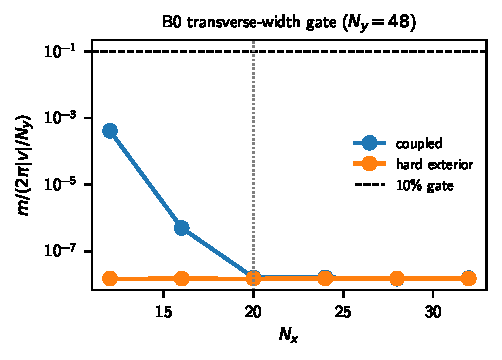
\includegraphics[width=0.48\textwidth]{../figures/width_convergence.pdf}
\caption{The hybridization-mass condition remains a necessary transverse-width gate.}
\end{figure}

\begin{figure}[h]
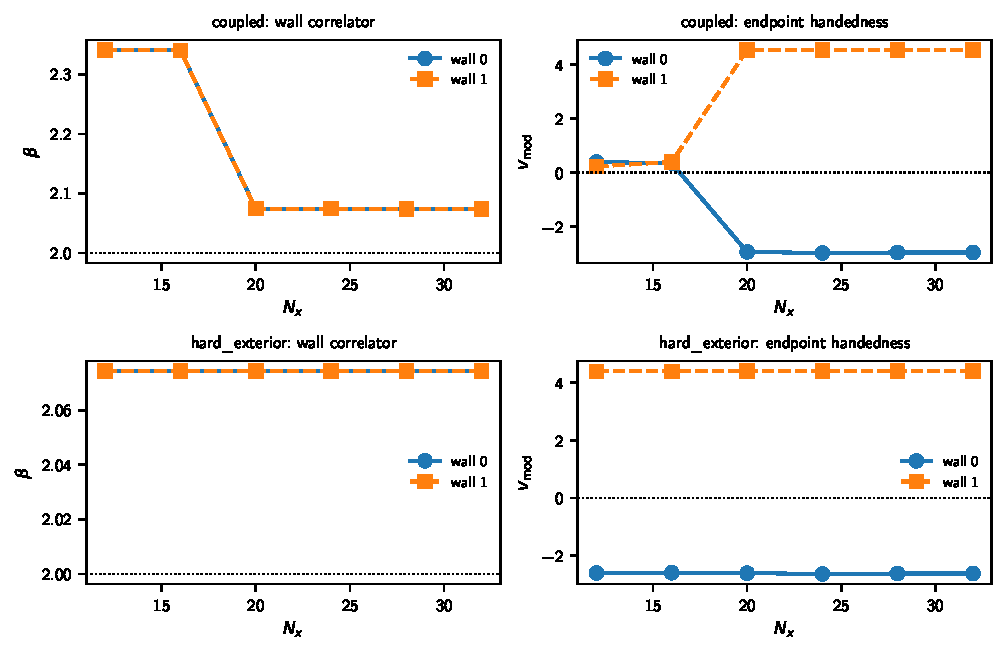
\includegraphics[width=0.80\textwidth]{../figures/local_calibration_convergence.pdf}
\caption{Local-observable convergence.  The coupled correlator and endpoint modular
handedness exclude $N_x=12,16$ even though their fitted hybridization masses pass.}
\end{figure}

\begin{figure}[h]
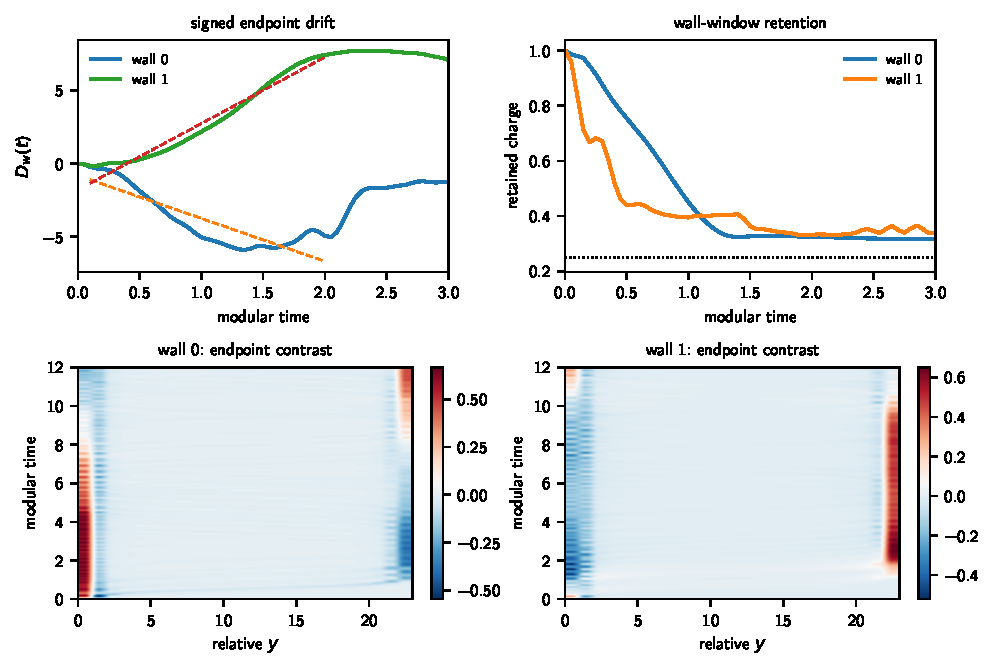
\includegraphics[width=0.48\textwidth]{../figures/modular_endpoint_drift__coupled.pdf}
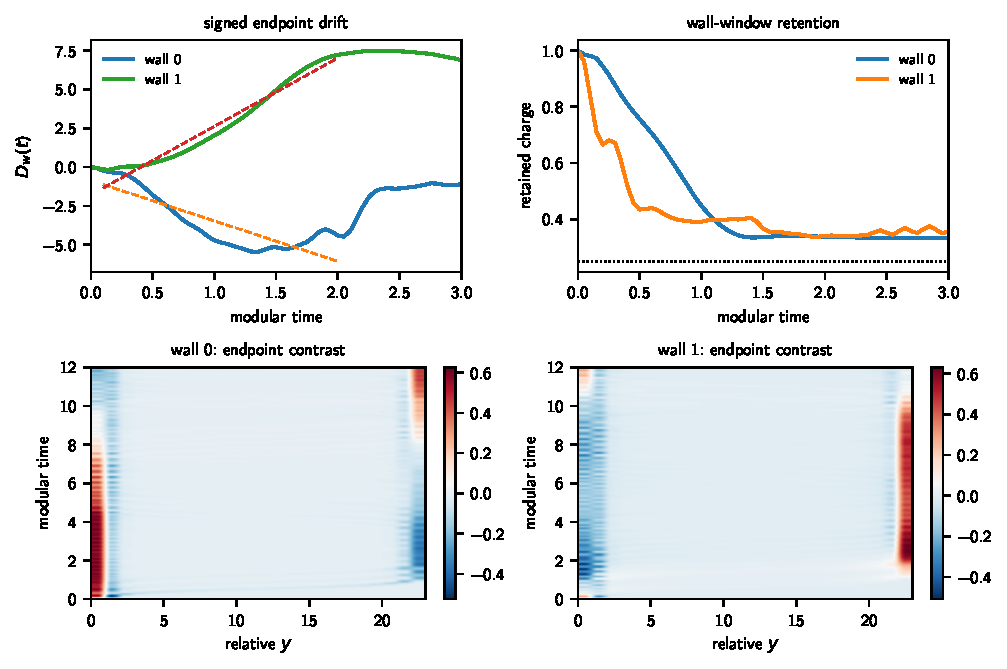
\includegraphics[width=0.48\textwidth]{../figures/modular_endpoint_drift__hard_exterior.pdf}
\caption{Separate entanglement-endpoint injections, signed drifts, and wall retention for
the accepted-width coupled and hard-exterior constructions.}
\end{figure}

\section{Entropy accounting}
The full-width strip has two entanglement boundaries and intersects both physical domain
walls.  Each three-column physical-wall contour window includes both entanglement cuts.
Those window sums are diagnostic contributions to the full entropy, not isolated subsystem
entropies.  The saved products test equality of the contour sum and the entropy, equality
of the two wall slopes, and the factor-of-two relation between a wall-window slope and the
full-strip slope.

\section{Acceptance ledger}
\begin{longtable}{p{0.36\textwidth}p{0.10\textwidth}p{0.46\textwidth}}
\toprule
requirement & status & details \\
\midrule
small-system formula and gauge preflight & PASS & completed before production stages \\
fixed-rank half filling & PASS & every geometry must contain exactly Nx Ny occupied orbitals \\
Hermiticity, projector, and contour numerics & PASS & absolute tolerance 1e-10 \\
consecutive full-calibration transverse-width gate & PASS & selected Nx=20; mass threshold 0.1; selected and next larger widths must pass every single-geometry gate \\
coupled: opposite, compatible spectral velocities & PASS & v0=-0.990726, v1=0.990726, relative mismatch=0 \\
coupled: finite transverse localization lengths & PASS & xi0=0.29557, xi1=0.29557 \\
coupled: Renyi q=1,2,3 full-strip c=1 & PASS & q=1: c=1.0001, q=2: c=0.99591, q=3: c=0.99336 \\
coupled: single-physical-wall contour factor of two & PASS & relative errors=[8.468181767162797e-05, 8.468181752530057e-05]; each window includes both entanglement cuts \\
coupled: wall squared-correlator exponent two & PASS & betas=[2.0744675989239347, 2.0744675989889787]; all four candidate models remain in correlator\_fits.csv \\
coupled: physical response chirality & PASS & response velocities=[-0.8720279720279717, 0.8720279720279717]; spectral velocities=[-0.9907263837597539, 0.9907263837597539]; relative magnitude errors=[0.11980947886068002, 0.11980947886068002] \\
coupled: response linearity and charge conservation & PASS & charge drift=2.21e-16; epsilon relative error=5e-07 \\
coupled: stable opposite endpoint modular velocities & PASS & primary velocities=[-2.930447164248109, 4.535630720918731]; sign stable=[True, True]; minimum retention=0.3245; norm drift=3.33e-15 \\
coupled: nonsingular overlap tracking & PASS & minimum singular value=0.999904 \\
coupled: unit wall flow and zero net flow & PASS & signed flows=[-1, 1] \\
hard\_exterior: opposite, compatible spectral velocities & PASS & v0=-0.990726, v1=0.990726, relative mismatch=0 \\
hard\_exterior: finite transverse localization lengths & PASS & xi0=0.222754, xi1=0.222754 \\
hard\_exterior: Renyi q=1,2,3 full-strip c=1 & PASS & q=1: c=1.0001, q=2: c=0.99591, q=3: c=0.99332 \\
hard\_exterior: single-physical-wall contour factor of two & PASS & relative errors=[8.629596877662848e-05, 8.629596836606801e-05]; each window includes both entanglement cuts \\
hard\_exterior: wall squared-correlator exponent two & PASS & betas=[2.074368474806555, 2.074368474815762]; all four candidate models remain in correlator\_fits.csv \\
hard\_exterior: physical response chirality & PASS & response velocities=[-0.8720279720279717, 0.8720279720279717]; spectral velocities=[-0.9907263837597539, 0.9907263837597539]; relative magnitude errors=[0.11980947886068002, 0.11980947886068002] \\
hard\_exterior: response linearity and charge conservation & PASS & charge drift=3.8e-16; epsilon relative error=5e-07 \\
hard\_exterior: stable opposite endpoint modular velocities & PASS & primary velocities=[-2.5998489202228035, 4.405780712633448]; sign stable=[True, True]; minimum retention=0.3349; norm drift=4e-15 \\
hard\_exterior: nonsingular overlap tracking & PASS & minimum singular value=0.999999 \\
hard\_exterior: unit wall flow and zero net flow & PASS & signed flows=[-1, 1] \\
33/65/129-point, both-sign, seam-relocation twist validation & PASS & all validation rows require unit absolute wall flow and seam/uniform spectral agreement \\
\bottomrule
\end{longtable}
The machine-readable ledger retains the same decisions and their thresholds.  Any failed
item remains explicit rather than changing the estimator or gate.
\end{document}
